%!TEX root = syntheyes15.tex

\section{Introduction}

\commentA{would be nice to show the process figure as a teaser above abstract as in the disney paper}
\commentE{Hmm I tried to abuse the title section to put the wide figure in, but this seems tricky. If you know anyone who's managed in MPII, let me know, I'm sure there's a way.}

Machine learning methods that leverage large amounts of training data currently perform best for many problems in computer vision, such as object detection, scene recognition, or gaze estimation~\cite{zhou2014learning,girshick2014rich,zhang15_cvpr}.
However, capturing or collecting large-scale training data can be extremely time-consuming, especially for new areas of research without pre-existing datasets.
In addition, supervised learning methods require accurate ground truth annotation for each image.
This annotation process can be expensive and tedious, and there is no guarantee that human-provided labels will be correct.
Ground truth annotation is particularly challenging and error-prone for learning tasks that require highly fine-grained and accurate labels, such as of facial landmarks for facial expression analysis and gaze estimation~\todo{REF} or body joints for pose estimation and activity recognition~\todo{REF}.

\begin{figure}
    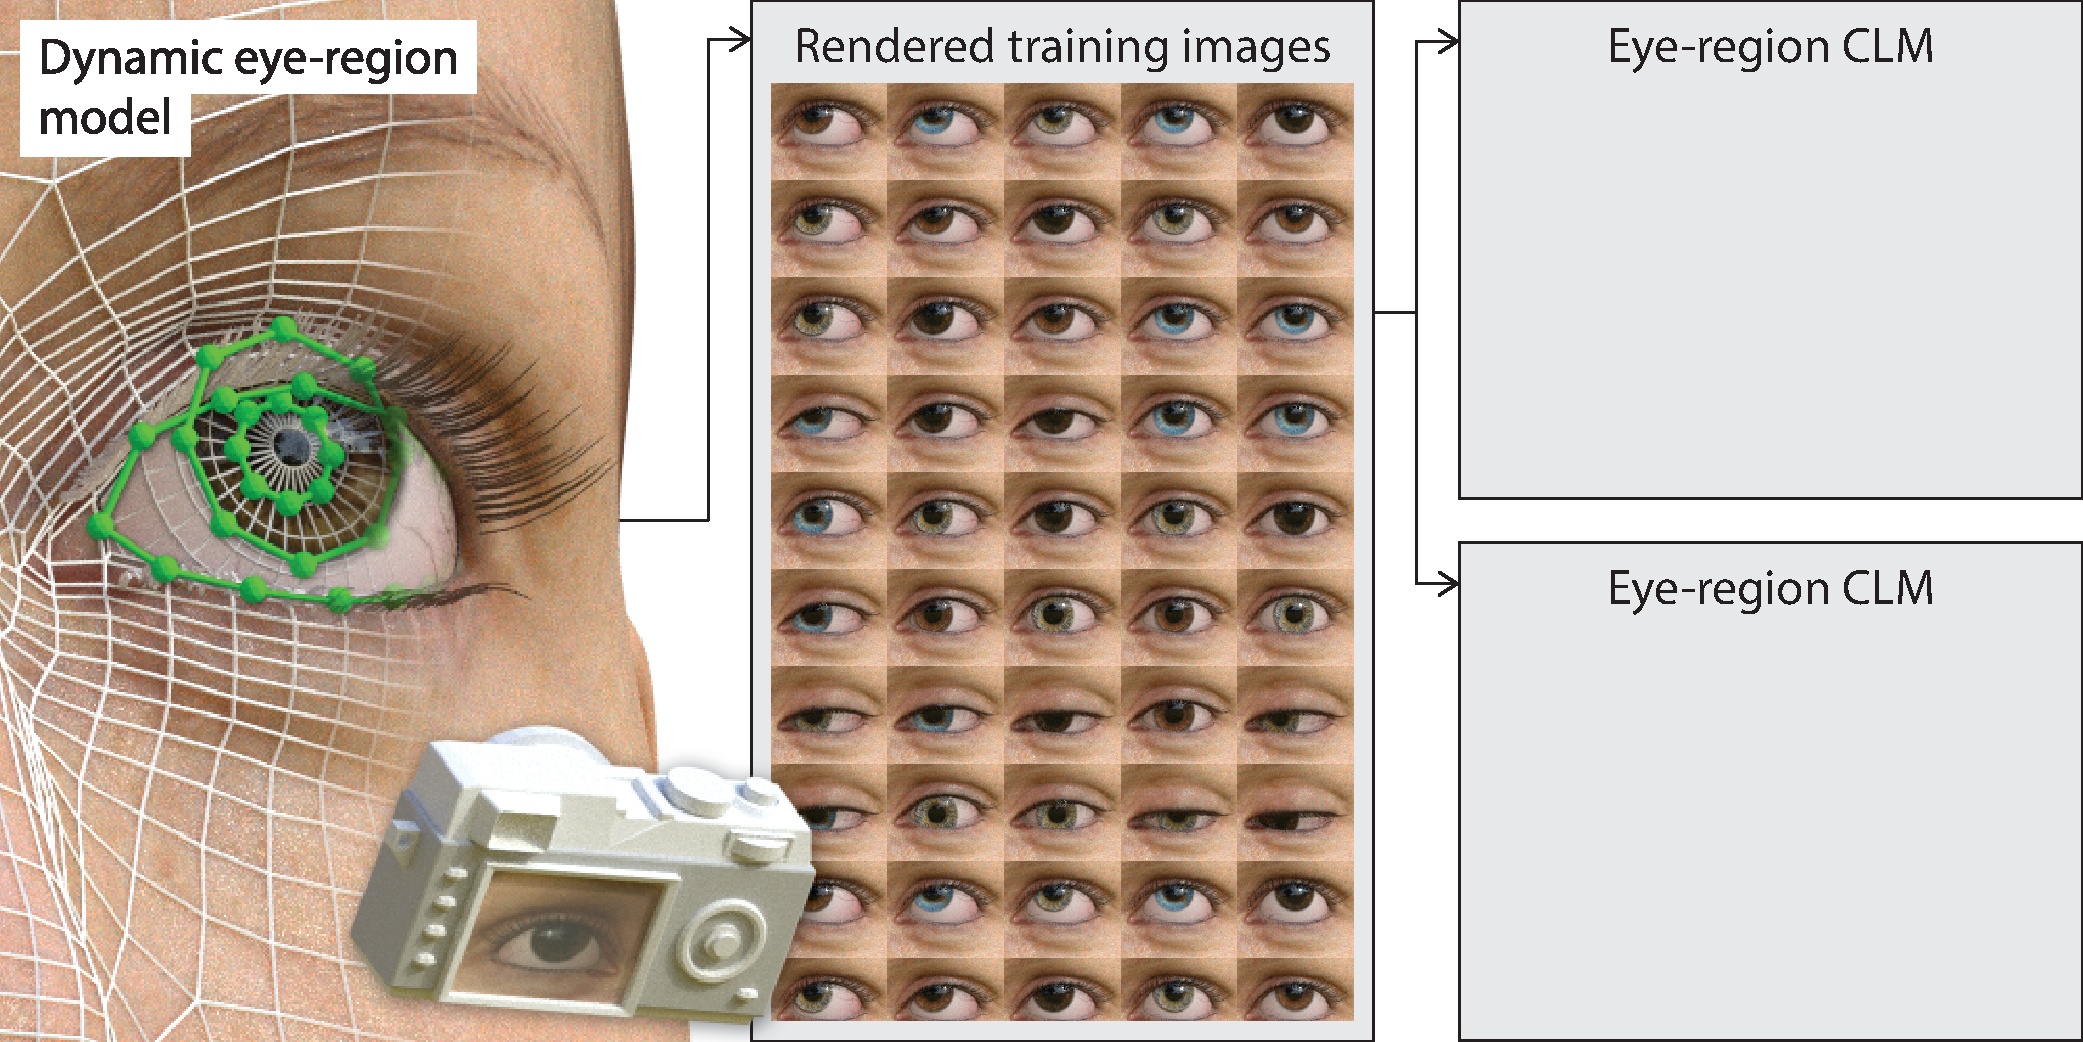
\includegraphics[width=\columnwidth]{main_img}
    \caption{We render images.}
    \label{fig:teaser}
\end{figure}

To address these problems, a number of recent works explored the potential of synthesising training images at a large scale.
The distinct advantages of this approach are that both data collection and annotation only require little human labour and image synthesis can be modified and geared to specific application scenarios.
For example, \todo{add example works without face and eye}
One area of the human body largely neglected in the context of image synthesis so far is the face and particularly the eyes.
This is partly due to these areas being particularly difficult to model accurately given the large amount of muscles and thus complex dynamic shape changes during different facial expressions and eyeball rotations, the large number of subtle details in appearance and texture around and in the eye, as well as the significant variation in general face and eye appearance across different people.
\todo{final sentence on limitations of existing models in this area}

% Andreas: we need some transition to eyeballs here, e.g. eyeball rendering is particularly challenging and interesting because of the many muscles involved, the large number of appearance details around and in the eye etc.
% essentially motivate that this hasn't been done before and is a very interesting area of research

%Synthesising training data is not novel in itself -- previous work has ... Our novel approach 

In this paper we present a novel method for photorealistic rendering of full face and eye images at a large scale.
Our method \todo{briefly summarise key characteristics of the method}
We describe how we prepare a collection of dynamic eye-region models, and then our approach for generating large amounts of photorealistic training data.
We then present and evaluate two separate systems trained on \dataset: a novel eye-region specific deformable model and an appearance-based gaze estimator.
These systems are case studies that show how we leverage the degrees of control made available by rendering our training data to easily and quickly generate high quality training datasets.
We show that by rendering all our training data, we achieve state of the art performance...

The specific contributions of this work are threefold. First, \todo{...}

